\section{Training System}
Training our \modelname~with 135B parameters on 13.2 trillion tokens necessitates the need to ensure training stability and efficiency in large-scale computing cluster.
In this section, we elaborate the details of our training system from two important perspectives: parallelization strategies and system-level optimization techniques, in Section~\ref{sec: parallelism} and Section~\ref{sec: sys-optimization}. 
Overall, we achieve over 52\% Model FLOPs Utilization (MFU) when training \modelname{} on 8,192 Ascend NPUs.




\subsection{Computing Setup}
A computing cluster with 8,192 Ascend Neural Processing Units (NPUs)~\cite{910b2, 910b2-technical} is deployed to train \modelname.
Each node in the cluster houses 8 NPUs, interconnected via Huawei Cache Coherence System (HCCS) using a full-mesh topology, and each device is equipped with 64GB Memory.
Inter-node communication is facilitated through RDMA over Converged Ethernet (RoCE) fabric, leveraging 200 Gbps interconnects for communication between NPUs across different nodes.

\subsection{Parallelism Strategies for Model Scaling}  \label{sec: parallelism}
In order to scale model training\footnote{The training of \modelname~is supported by MindSpeed \cite{mindspeed} and Megatron \cite{megatron-github, megatron-lm} framework, which provides comprehensive parallel strategies and system optimization methods.}, we leverage a combination of different parallelism strategies to distributes the model across multiple NPUs, including Data Parallelism (DP) \cite{data_parallel}, Tensor Parallelism (TP) \cite{megatron-lm}, Sequence Parallelism (SP) \cite{megatron-sp}, and Pipeline Parallelism (PP) \cite{gpipe, pipedream}.
For \modelname, 128-way DP with ZERO \cite{zero} is performed to reduce the memory cost of model parameters and the associated optimizer states. 
8-way TP is applied to leverage the high intra-node bandwidth for efficient activation transfer, while 8-way PP is adopted to utilize inter-node connections, since it only requires transmitting activations at the partition boundaries.
However, as mentioned in existing studies \cite{megascale, gpipe, pipedream, zero_pp}, pipeline parallelism encounters severe PP bubbles when the training cluster scales up, primarily due to batch size constraints \cite{megascale}.
For one-forward-one-backward (1F1B) PP scheduling, the bubble ratio is defined as $\frac{p-1}{p-1+n}$, where $p$ represents the number of pipeline stages and $n$ denotes the number of micro batches for every DP. The ratio represents the idle time of accelerators, as shown in Figure \ref{fig:interleaved-pp}.
A large-scale training cluster increases the number of DPs, which in turn reduces the number of micro batches assigned to each DP due to batch size constraints, leading to a significant increase in the bubble ratio.
Therefore, minimizing bubble ratio is crucial for improving system efficiency.
Under such circumstances, we employ interleaved pipeline-parallel scheduling with 6-way virtual PP stages on each device~\cite{interleaved-pp} and manage to reduce it from 30.45\% to 6.8\%. 
Through careful tuning of load balancing across PP and VPP stages, we are able to achieve approximately 43\% MFU on an 8,192 NPU cluster as a baseline.

\begin{figure}[htbp]
    \centering
    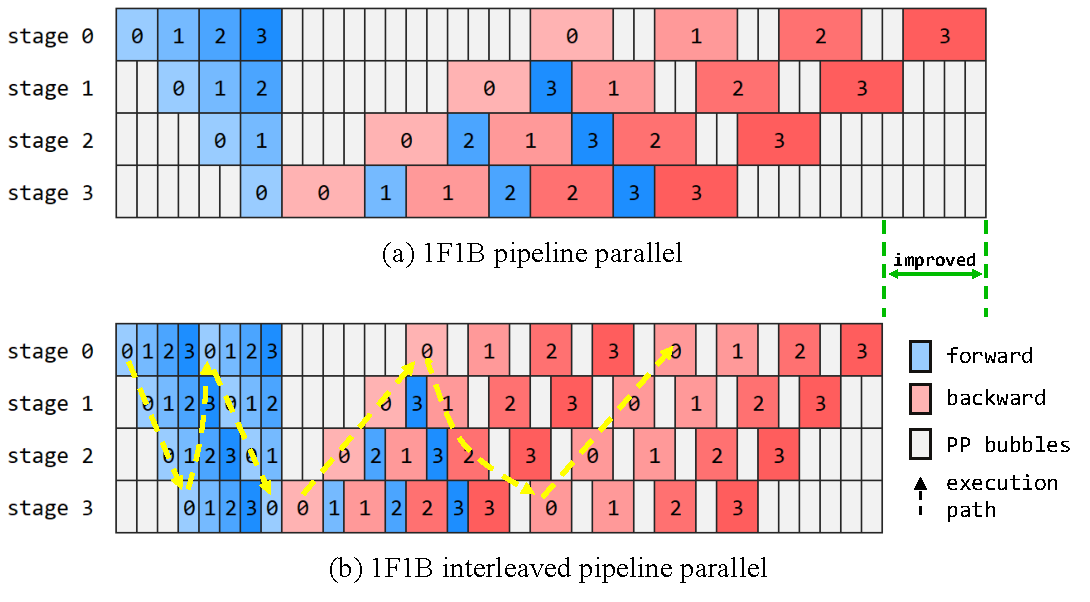
\includegraphics[width=0.8\textwidth]{fig/pipeline_parallelism.pdf}
    \caption{Pipeline parallelism and the interleaved pipeline-parallel scheduling.}
    \label{fig:interleaved-pp}
\end{figure}

\subsection{System Optimization}\label{sec: sys-optimization}

Based on the optimizations outlined in Section \ref{sec: parallelism} that achieved 43\% MFU, additional system-level enhancements are implemented to push training efficiency to new heights. 
Through a combination of kernel fusions, context parallelism via subsequence partitioning, data caching and sharing mechanisms, and other refinements, \modelname~benefits from a significant improvement in training efficiency.
These comprehensive optimizations enable the system to achieve over 52\% MFU, representing a 9\% relative improvement compared to the baseline configuration mentioned in Section \ref{sec: parallelism}.

\begin{figure}[htbp]
    \centering
    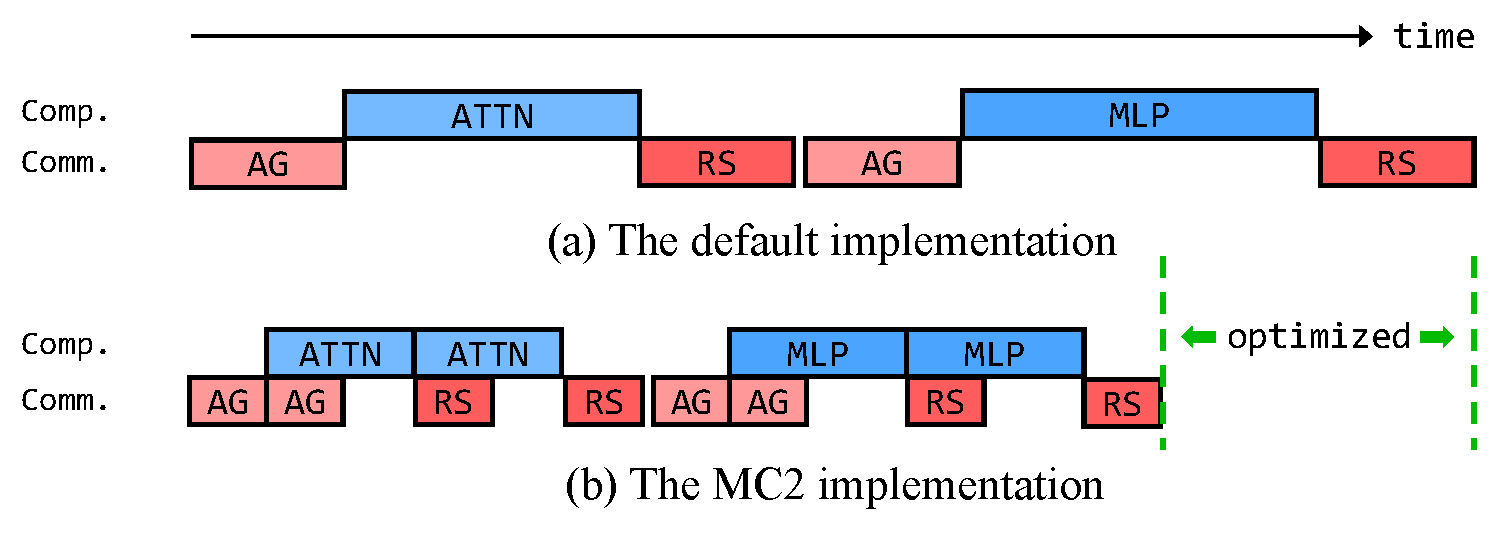
\includegraphics[width=0.7\textwidth]{fig/the_mc2.pdf}
    \caption{A Comparison of the default transformer computation and the MC2 method. Note that in actual training, communication and computation tasks are fused into a single kernel in MC2.} 
    \label{fig:mc2}
\end{figure}

\subsubsection{Kernel Fusion}
Kernel fusion is widely adopted in LLM training to enhance efficiency. It combines multiple operations into a single kernel, reducing the number of data accesses to global memory \cite{flash_attention2}. 
During the training phase of \modelname, key operators are fused, resulting in significant improvements in hardware utilization and overall training efficiency.


\textbf{MC2 - Merged Compute and Communication} 
Tensor parallelism, when combined with sequence parallelism, introduces All-Gather (AG) and Reduce-Scatter (RS) communication operations for exchanging input and output activations across distributed devices.
This approach exhibits a direct dependency between matrix multiplication (MatMul) and AG/RS communications, which fundamentally constrains the overlapping of TP communication with computational workflows.
The MC2 is implemented \cite{ascend_mc2, mc2} to tackle this challenge by fusing MatMul computations with communication operations.
It decomposes large computation and communication tasks into fine-grained subtasks and employs pipelined execution to maximize overlap between communication and computation. 
Thus, MC2 significantly reduces communication latency and improves hardware utilization (Figure \ref{fig:mc2}).

\textbf{NPU Fusion Attention}
Training LLMs with long sequence length suffers from quadratic memory and computational requirements in self-attention mechanisms as sequence length grows. 
To address these challenges, Flash Attention (FA) has emerged as a standard technique in LLM training owing to its superior performance \cite{flash_attention, flash_attention2}.
\modelname~ leverages a self-attention fusion operator, called NPU Fusion Attention (NFA)\cite{npu_fa}, which is specifically optimized for Ascend NPUs, offering system-level improvements across a wide range of self-attention computation scenarios.
\begin{figure}[htbp]
    \centering
    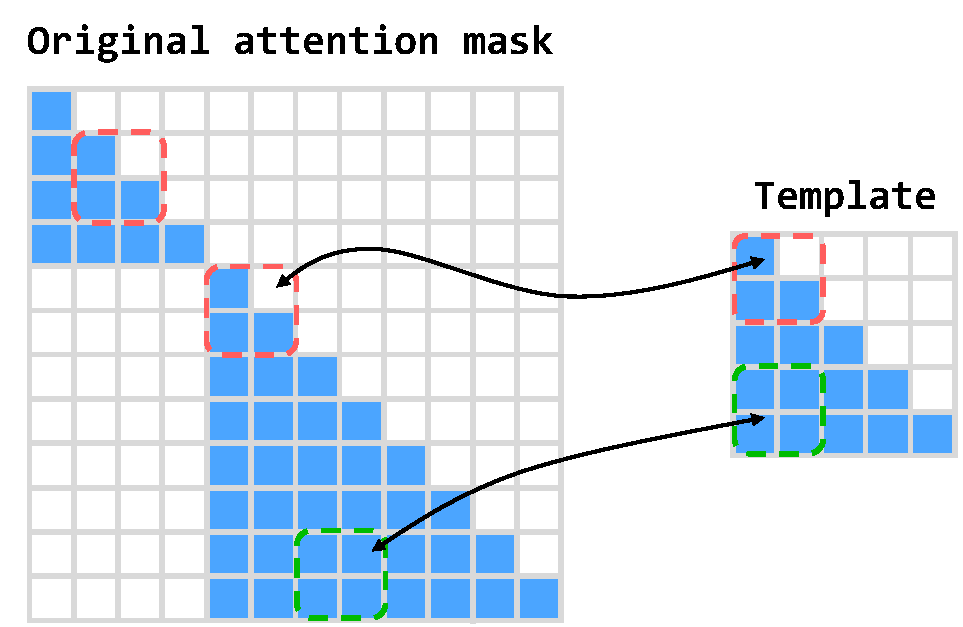
\includegraphics[width=0.4\textwidth]{fig/atten_mask_compression.pdf}
    \caption{Examples of attention mask compression for the NFA operator.}
    \label{fig:attn_mask_compression}
\end{figure}

It is worth mentioning that \modelname~uses a reset attention mask strategy to prevent self-attention between different documents within a sequence.
This requires calculating the corresponding attention mask for every sequence, leading to significant memory and computational overhead.
To mitigate the time and memory requirements of generating attention masks, the NFA operator employs a mask compression optimization.
As shown in Figure \ref{fig:attn_mask_compression}, NFA utilizes a $2048 \times 2048$ causal mask as a template to construct the computational mask within the fusion attention operator.
For every iteration, \modelname~ retrieves the actual sequence length based on the position of the end-of-document (eod) token, which is then provided as input to the NFA operator to accelerate the computation of self-attention.
The detailed usage of NFA is provided in the Ascend documentation~\cite{npu_fa}.

\textbf{Other Kernel Fusions for Efficiency} 
In addition to MC2 and NPU-optimized fused attention, we also integrate a series of kernel fusion optimizations within key components such as RMSNorm \cite{zhang2019rootmeansquarelayer}, SwiGLU \cite{shazeer2020glu}, and rotary positional embeddings (RoPE) \cite{su2023roformerenhancedtransformerrotary}, as well as critical processes including gradient accumulation and PP send/receive communications.
These fusion operators are designed to reduce kernel launch and memory access overheads, while maintaining high numerical precision and enhancing overall training performance.

\begin{figure}[htbp]
    \centering
    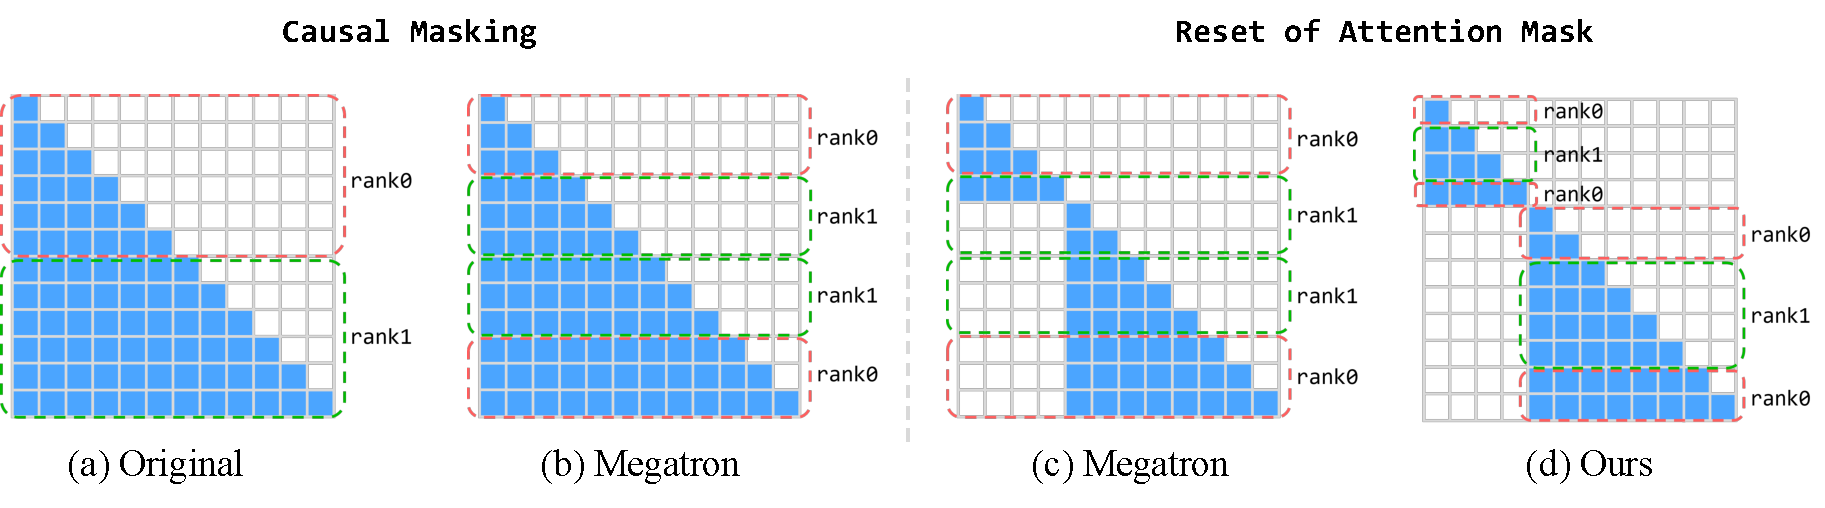
\includegraphics[width=\textwidth]{fig/sub_seq_partition.pdf}
    \caption{Examples of the mechanism of sub-sequence partitioning for context parallelism.}
    \label{fig:sub_seq_partition}
\end{figure}

\subsubsection{Optimization for Long Context Training}
Scaling long-context capabilities is becoming increasingly important for applications such as long document summarization and conversational AI.
However, training on long sequences presents several challenges in terms of both time and memory complexity.
To improve the efficiency of long-context training, we propose two key strategies, as outlined below.

\textbf{Sub-Sequence Partitioning for Context Parallelism} 
Context parallelism (CP) is an crucial approach for the training of very long sequences, that divides the input sequence into segments to reduce memory consumption \cite{ringattention, ulysses}.
Yet, with causal masking, simply splitting the sequence into $CP$ chunks results in a severely imbalanced workload for Ring Self-Attention (RSA) \cite{ringattention} (as shown in Figure \ref{fig:sub_seq_partition}(a)).
Megatron-LM addresses this issue by splitting the sequence into $2\times CP$ chunks, where each rank receives chunks from both the top and bottom, thus balancing the workload within a CP group (Figure \ref{fig:sub_seq_partition}(b)) \cite{megatron-github}.
However, this method still results in an imbalanced workload when the attention mask is reset (Figure \ref{fig:sub_seq_partition}(c)).
Therefore, in training with 128k-long contexts, we propose a load-balanced partitioning strategy for CP training, where each rank is responsible for computing two chunks within each subsequence (Figure \ref{fig:sub_seq_partition}(d)).

\textbf{Fast Mask Generation and Data Reuse}
When scaling the training sequence of \modelname~up to 128k, the generation of the attention mask or the calculation of the actual sequence length still incurs a non-negligible performance overhead.
Additionally, in the training scenario with reset attention masks, each VPP stage is required to retrieve the corresponding mask or actual sequence length in every iteration, resulting in redundant computations and increased overhead.
We optimize these problems by (1) using efficient NPU operators to compute the attention mask, instead of constructing it on the CPU, thus accelerating mask generation and eliminating the need for data transfer between the CPU and NPU, and (2) enabling cross-VPP stage mask sharing, where attention masks are generated by the first stage (VPP0) and shared across different VPP stages on the same rank, thereby avoiding redundant mask computations and memory cost.